\documentclass[letter,11pt]{article}

\usepackage[spanish,es-nodecimaldot]{babel}
\usepackage[utf8]{inputenc}

\usepackage{lmodern}
\usepackage[T1]{fontenc}
\usepackage{textcomp}

\usepackage{framed}
\usepackage[svgnames]{xcolor}
\colorlet{shadecolor}{Gainsboro!50}

\usepackage[labelfont=bf]{caption}
\usepackage{graphicx}
\usepackage{pstricks}

\usepackage{anysize}
\marginsize{3cm}{2cm}{2cm}{3cm}

\usepackage{siunitx}
\usepackage{amsmath}
\usepackage{array}
\usepackage{csquotes}

\usepackage{fancyhdr}
\usepackage{lastpage}
\pagestyle{fancy}
\fancyhf{}
\fancyhead[LE,RO]{Laboratorio de Circuitos Eléctricos I}
\fancyfoot[CO,CE]{\thepage\ de \pageref{LastPage}}

\special{papersize=215.9mm,279.4mm}

\usepackage[
    pdfauthor={Carlos Eduardo Caballero Burgoa},%
    pdftitle={Laboratorio de Circuitos Eléctricos I},%
    pdfsubject={Potencia y máxima transferencia de potencia},%
    colorlinks,%
    citecolor=black,%
    filecolor=black,%
    linkcolor=black,%
    urlcolor=black,
    breaklinks]{hyperref}
\usepackage{breakurl}

\newcommand{\blankpage}{
\newpage
\thispagestyle{empty}
\mbox{}
\newpage
}

\renewcommand{\arraystretch}{1.2}

\begin{document}

\begin{titlepage}
    \begin{center}
        {\Large UNIVERSIDAD MAYOR DE SAN SIMÓN}\\
        \vspace*{0.15cm}
        {\large FACULTAD DE CIENCIAS Y TECNOLOGÍA}\\
        \vspace*{0.10cm}
        DEPARTAMENTO DE ELÉCTRICA-ELECTRÓNICA\\
        \vspace*{3.0cm}
        {\Large \textbf{LABORATORIO DE CIRCUITOS ELÉCTRICOS I}}\\
        \vspace*{0.3cm}
        {\Large \textbf{INFORME No. 5}}\\
        \vspace*{3.5cm}
        {\Large \textbf{POTENCIA Y MÁXIMA \\ TRANSFERENCIA DE POTENCIA}}\\
    \end{center}

    \vspace*{5.8cm}
    \leftskip=7.95cm
    \noindent
    \textbf{Estudiante:}\\
    Caballero Burgoa, Carlos Eduardo.\\
    \newline
    \textbf{Carrera:}\\
    Ing. Electromecánica.\\
    \newline
    \textbf{Docente:}\\
    Ing. Marco Antonio Vallejo Camacho.\\
    \newline
    \textbf{Grupo:} 3E.\\
    \textbf{Fecha de entrega:} 28 de Mayo del 2024.\\
\end{titlepage}

\section{Cálculos previos}

\vspace{2.0cm}
\begin{figure}[!h]
\centering
\includegraphics[scale=0.18]{resources/preinforme1.eps}
\end{figure}

\newpage

\begin{figure}[!h]
\centering
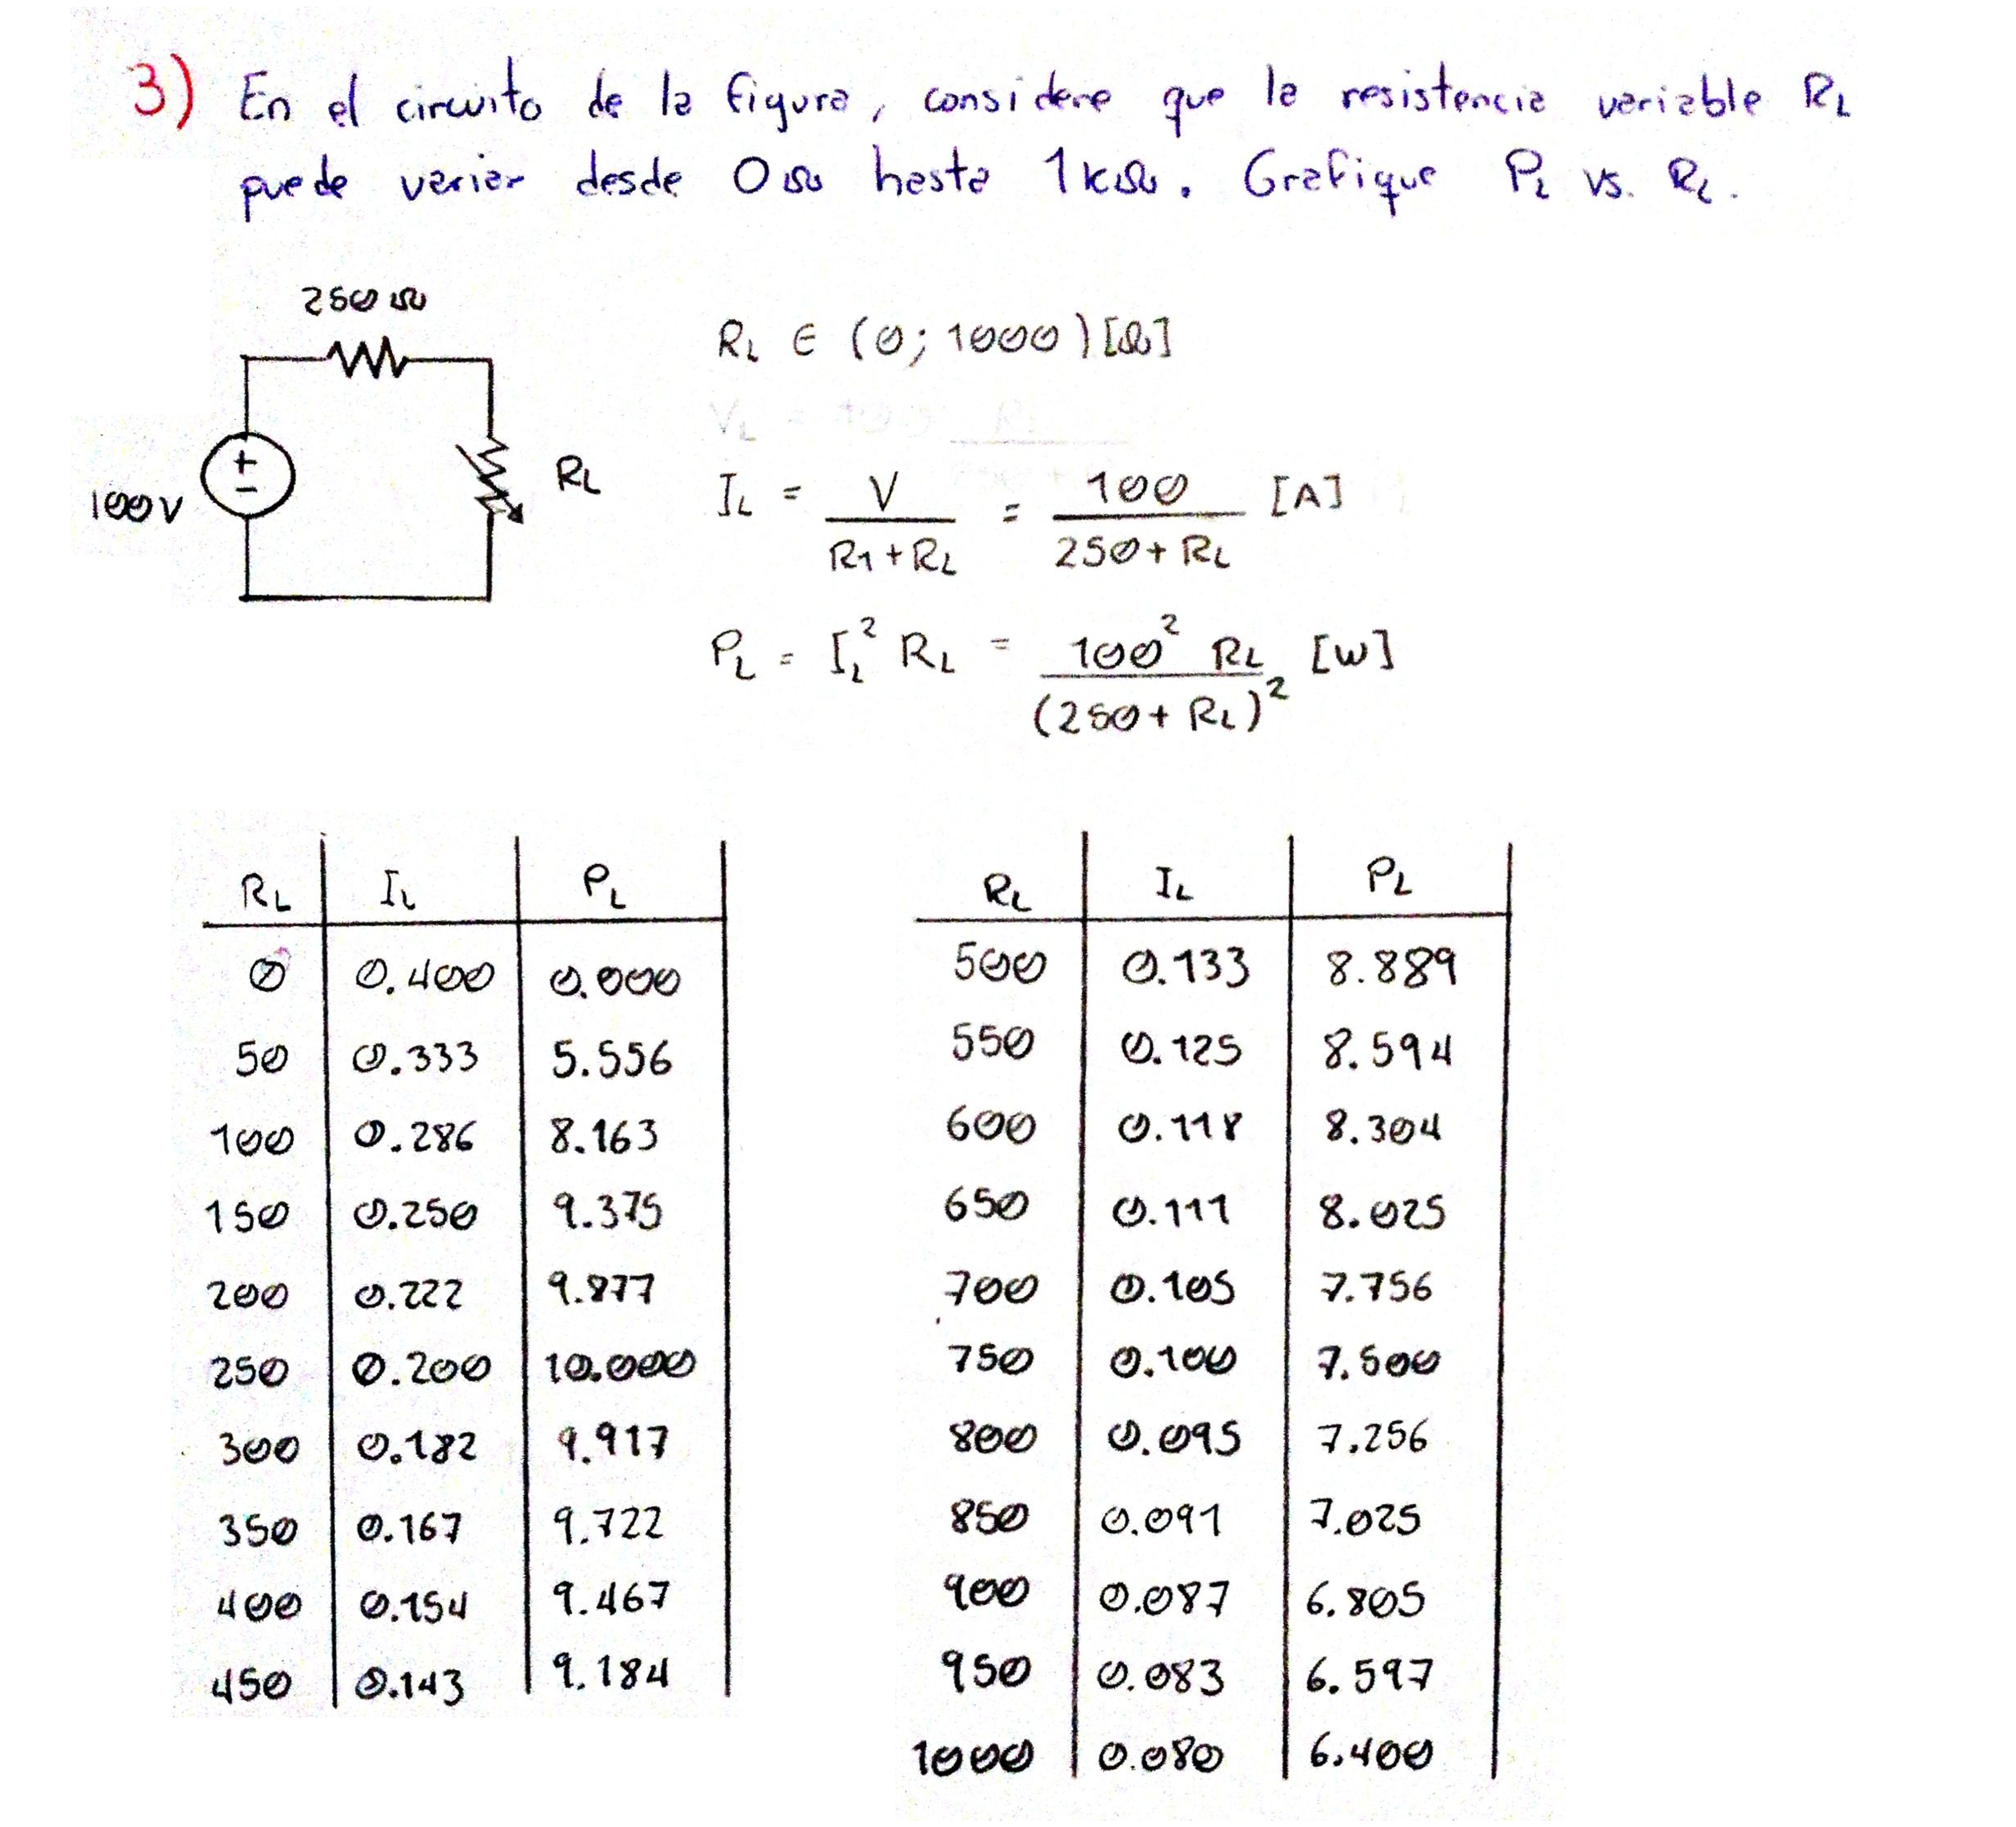
\includegraphics[scale=0.18]{resources/preinforme2.eps}
\end{figure}

\newpage

\begin{figure}[!h]
\centering
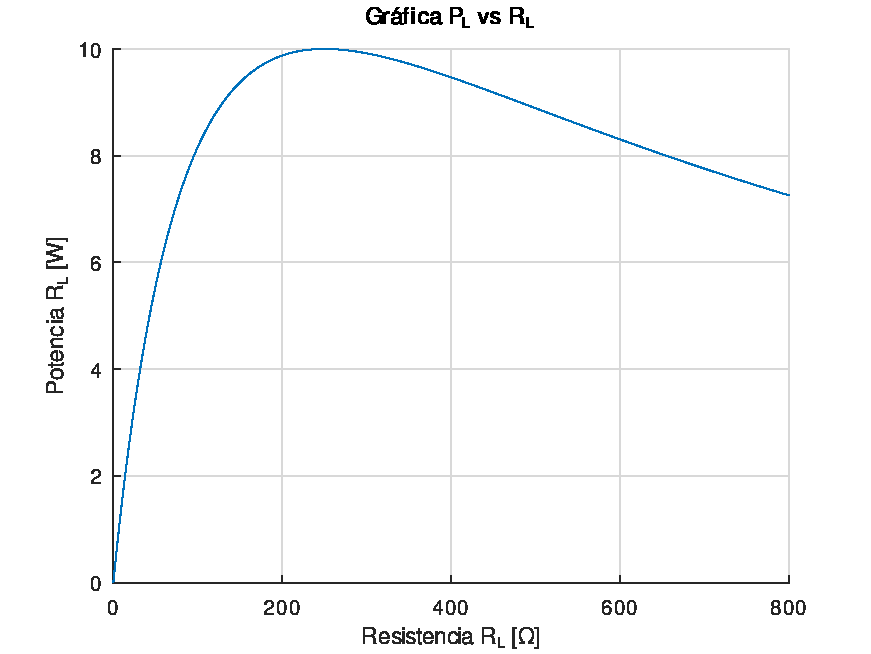
\includegraphics[scale=0.80]{simulation/grafica.eps}
\end{figure}

\section{Simulación}
Se utilizó el software \emph{Quite Universal Circuit Simulator.} para simular
el circuito, este puede verse en la figura (\ref{simulacion1}).

\begin{figure}[!h]
\centering
\includegraphics[scale=0.95]{simulation/practica5.eps}
\caption{Simulación del circuito para calculo de potencias.}
\label{simulacion1}
\end{figure}

\newpage

\section{Tablas y mediciones}
En la figura (\ref{tablas}), se adjunta la hoja de resultados provista en la
guía de laboratorio, rellenada con la información teórica, simulada y las
mediciones realizadas en laboratorio.

\begin{figure}[!h]
\centering
\includegraphics[scale=0.18]{resources/preinforme3.eps}
\caption{Tabla de resultados.}
\label{tablas}
\end{figure}

\section{Cuestionario}

\begin{enumerate}

\item \textbf{Con los datos presentados en la tabla 5.2, verifique la
conservación de la energía.}

Los valores de potencia son los siguientes:

\begin{center}
\begin{tabular}{|c|c|c|c|c|}
\hline
\textbf{Medición} & $V_S [W]$ & $R_1 [W]$ & $R_2 [W]$ & $R_3 [W]$
\tabularnewline \hline \hline
Calculo teórico & 57.14 & 40.82 & 13.06 & 3.26 \tabularnewline \hline
Voltaje x corriente & 48.62 & 35.256 & 11.13 & 2.682 \tabularnewline \hline
Vatímetro & 62 & 44 & 14 & 3 \tabularnewline \hline
\end{tabular}
\end{center}

Para verificar la conservación de la energía, la potencia disipada por las
resistencias debe ser igual a la potencia suministrada por la fuente de voltaje:
\\

\underline{Calculo teórico}:\\
\begin{equation*}
    P_{\text{dis}} = 40.82 + 13.06 + 3.26 = 57.14 [W] = P_{\text{sum}}
\end{equation*}

\underline{Voltaje x corriente}:\\
\begin{equation*}
    P_{\text{dis}} = 35.256 + 11.13 + 2.682 = 49.068 [W] \approx 48.62 [W]
\end{equation*}
\begin{equation*}
    \text{Error} = \frac{49.068 - 48.62}{48.62} * 100 = 0.92 \%
\end{equation*}

\underline{Vatímetro}:\\
\begin{equation*}
    P_{\text{dis}} = 44 + 14 + 3 = 61 [W] \approx 62 [W]
\end{equation*}
\begin{equation*}
    \text{Error} = \frac{62 - 61}{62} * 100 = 1.61 \%
\end{equation*}

Ambas discrepancias están dentro de los margenes de error de la medición.

\item \textbf{Si consideramos un circuito como el mostrado en la figura a
continuación se puede encontrar que la potencia consumida en la resistencia de
carga $R_L$ esta dada por la ecuación presentada en la misma figura. Demostrar
matemáticamente el teorema de la máxima transferencia de potencia
($R_L = R_S$).}\\

\begin{figure}[!h]
\centering
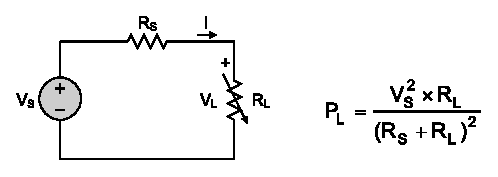
\includegraphics[width=0.55\textwidth]{resources/figura1.eps}
\end{figure}

Se calcula el voltaje de la resistencia $R_L$ a partir del divisor de tensión:
\begin{equation}
    V_L = V_S\,\frac{R_L}{R_S + R_L}
    \label{vl}
\end{equation}

Se calcula la corriente de la resistencia $R_L$ a partir de la ley de
\emph{Ohm}:
\begin{equation}
    I_L = \frac{V_S}{R_{eq}} = \frac{V_S}{R_S + R_L}
    \label{il}
\end{equation}

Se halla la potencia de la resistencia $R_L$ haciendo uso de las ecuaciones
(\ref{vl}) y (\ref{il}):
\begin{equation*}
    \begin{split}
        P_L &= I_L\,V_L \\
            &= \frac{V_S}{R_S + R_L}\,V_S\,\frac{R_L}{R_S + R_L} \\
    \end{split}
\end{equation*}
\begin{equation}
    P_L = V_S^2\,\frac{R_L}{(R_S + R_L)^2}
    \label{pl}
\end{equation}

Para hallar el máximo de la función se calcula la derivada de (\ref{pl}) y se
iguala a $0$:
\begin{equation*}
    \begin{split}
        \frac{dP_L}{dR_L} = \left(V_S^2\,\frac{R_L}{(R_S + R_L)^2}\right)^{'} \\
            0 = V_S^2\,\left(\frac{R_L}{(R_S + R_L)^2}\right)^{'} \\
            0 = V_S^2\,\left(\frac{R_L'}{(R_S + R_L)^2} + \frac{R_L}{[(R_S + R_L)^2]^{'}}\right) \\
            0 = V_S^2\,\left(\frac{1}{(R_S + R_L)^2} - \frac{2\,R_L}{(R_S + R_L)^3}\right) \\
            \frac{1}{(R_S + R_L)^2} = \frac{2\,R_L}{(R_S + R_L)^3} \\
            R_S + R_L = 2\,R_L \\
    \end{split}
\end{equation*}
\begin{equation}
    R_S = R_L
    \label{rl}
\end{equation}

\item \textbf{Graficar $P_L$ vs. $R_L$ empleando los resultados obtenidos en la
tabla 5.3. Verifique en que valor de $R_L$ se da la máxima transferencia de
potencia.}\\

\begin{figure}[!h]
\centering
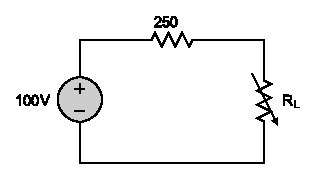
\includegraphics[width=0.32\textwidth]{resources/figura2.eps}
\end{figure}

Los datos medidos son:
\begin{center}
\begin{tabular}{|c|c|c|}
\hline
\textbf{Nº} & $R_L$ & $P_L$ \tabularnewline \hline \hline
 1 & 748.00 &  7.48 \tabularnewline \hline
 2 & 646.36 &  7.82 \tabularnewline \hline
 3 & 506.15 &  8.55 \tabularnewline \hline
 4 & 377.50 &  9.66 \tabularnewline \hline
 5 & 310.00 & 10.04 \tabularnewline \hline
 6 & 251.50 & 10.06 \tabularnewline \hline
 7 & 221.43 &  9.76 \tabularnewline \hline
 8 & 184.35 &  9.75 \tabularnewline \hline
 9 & 161.25 &  9.29 \tabularnewline \hline
10 & 144.00 &  9.00 \tabularnewline \hline
11 & 122.96 &  8.96 \tabularnewline \hline
\end{tabular}
\end{center}

\begin{figure}[!h]
\centering
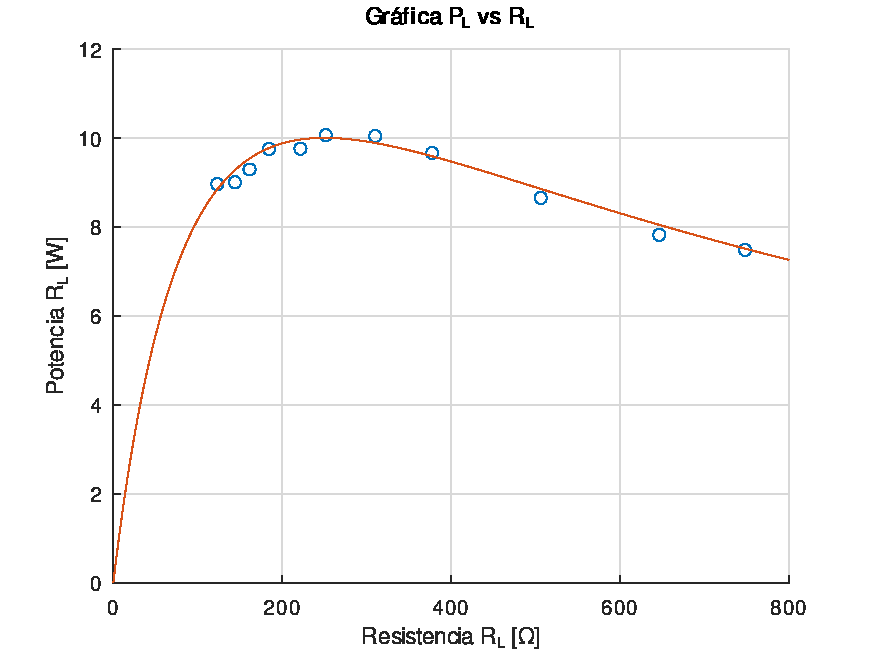
\includegraphics[width=0.80\textwidth]{resources/o1.eps}
\caption{Curva de potencia y valores tomados en laboratorio.}
\label{plvsrl}
\end{figure}

En la figura (\ref{plvsrl}) se muestra la curva de la función potencia y los
datos tomados en laboratorio, puede apreciarse que la máxima transferencia de
potencia se realizó en la muestra $6$, cuyo valor de resistencia es
$251.51 [\Omega]$ para la cual la potencia es $10.06 [W]$.

\end{enumerate}

\section{Conclusiones}
En laboratorio se realizaron mediciones de potencia con la ayuda de multímetros
para la toma de tensión y corriente, además haciendo uso del vatímetro, si bien
en las mediciones de potencia se pudo constatar la conservación de energía, los
valores son diferentes.

\begin{center}
\begin{tabular}{|c|c|c|c|}
\hline
& \textbf{Voltaje x corriente} & \textbf{Vatímetro} & \textbf{Error}
\tabularnewline \hline \hline
$V_S$ & 48.62 & 62 & $21.58\%$ \tabularnewline \hline
$R_1$ & 35.26 & 44 & $19.86\%$ \tabularnewline \hline
$R_2$ & 11.13 & 14 & $20.50\%$ \tabularnewline \hline
$R_3$ &  2.68 &  3 & $10.67\%$ \tabularnewline \hline
\end{tabular}
\end{center}

Esta discrepancia puede deberse a la forma de medición, ya que la medición con
vatímetro se realizo en cuatro etapas (una componente a la vez), mientras que
la medición con multímetros se realizo en dos etapas (conectando hasta cuatro
multímetros a la vez en el circuito). Por lo cual el voltaje de regulación de la
fuente ha podido caer por debajo del valor real.

Entonces la medición con vatímetro debe estar mas próximo al valor real de
potencia.
\\

Adicionalmente se comprobó teóricamente y en laboratorio la máxima potencia
que es transferida a una resistencia y como tal valor máximo esta relacionado
con la resistencia de \emph{Thévenin}.

\end{document}

